\documentclass[../react]{subfiles}
\begin{document}
	
	\section{Architecture}

	Reacts make it easy to build UI by dividing into components each part of your frontend views.
	Marvin is split up in 4 different types of components:
	\begin{enumerate} 
		\item \textbf{Bootstrap Components};
		\item \textbf{Custom Components};
		\item \textbf{Page templates and routes};
		\item \textbf{User pages instances}.
	\end{enumerate} 

	\subsection{Props}
	React components implement a render method that takes input data and returns what to display.
	Input data that is passed to the component as props and can be accessed via this.props.

	\subsection{State}
	Build encapsulated components that manage their own state, then compose them to make complex UIs.

	\subsection{Store}
	Only the final components, user page instances, will have a different kind of source of data, being the store.
	The store is handled by Redux with a React-Redux connection plugin.
	
	\subsection{UML} %TODO ricordo di mettere diagramma aggiornato architettura!!
	
	\textbf{Architecture Packages Overview}
	\begin{figure}[H]
		\centering
		\includegraphics[width=1\linewidth]{"../diagrammi/react/simplearch"}
		\caption{Simple React Architecture}
		\label{fig:Simple React Architecture}
	\end{figure}
	
	\newpage
	\textbf{Entire architecture overview}
	\begin{figure}[H]
		\centering
		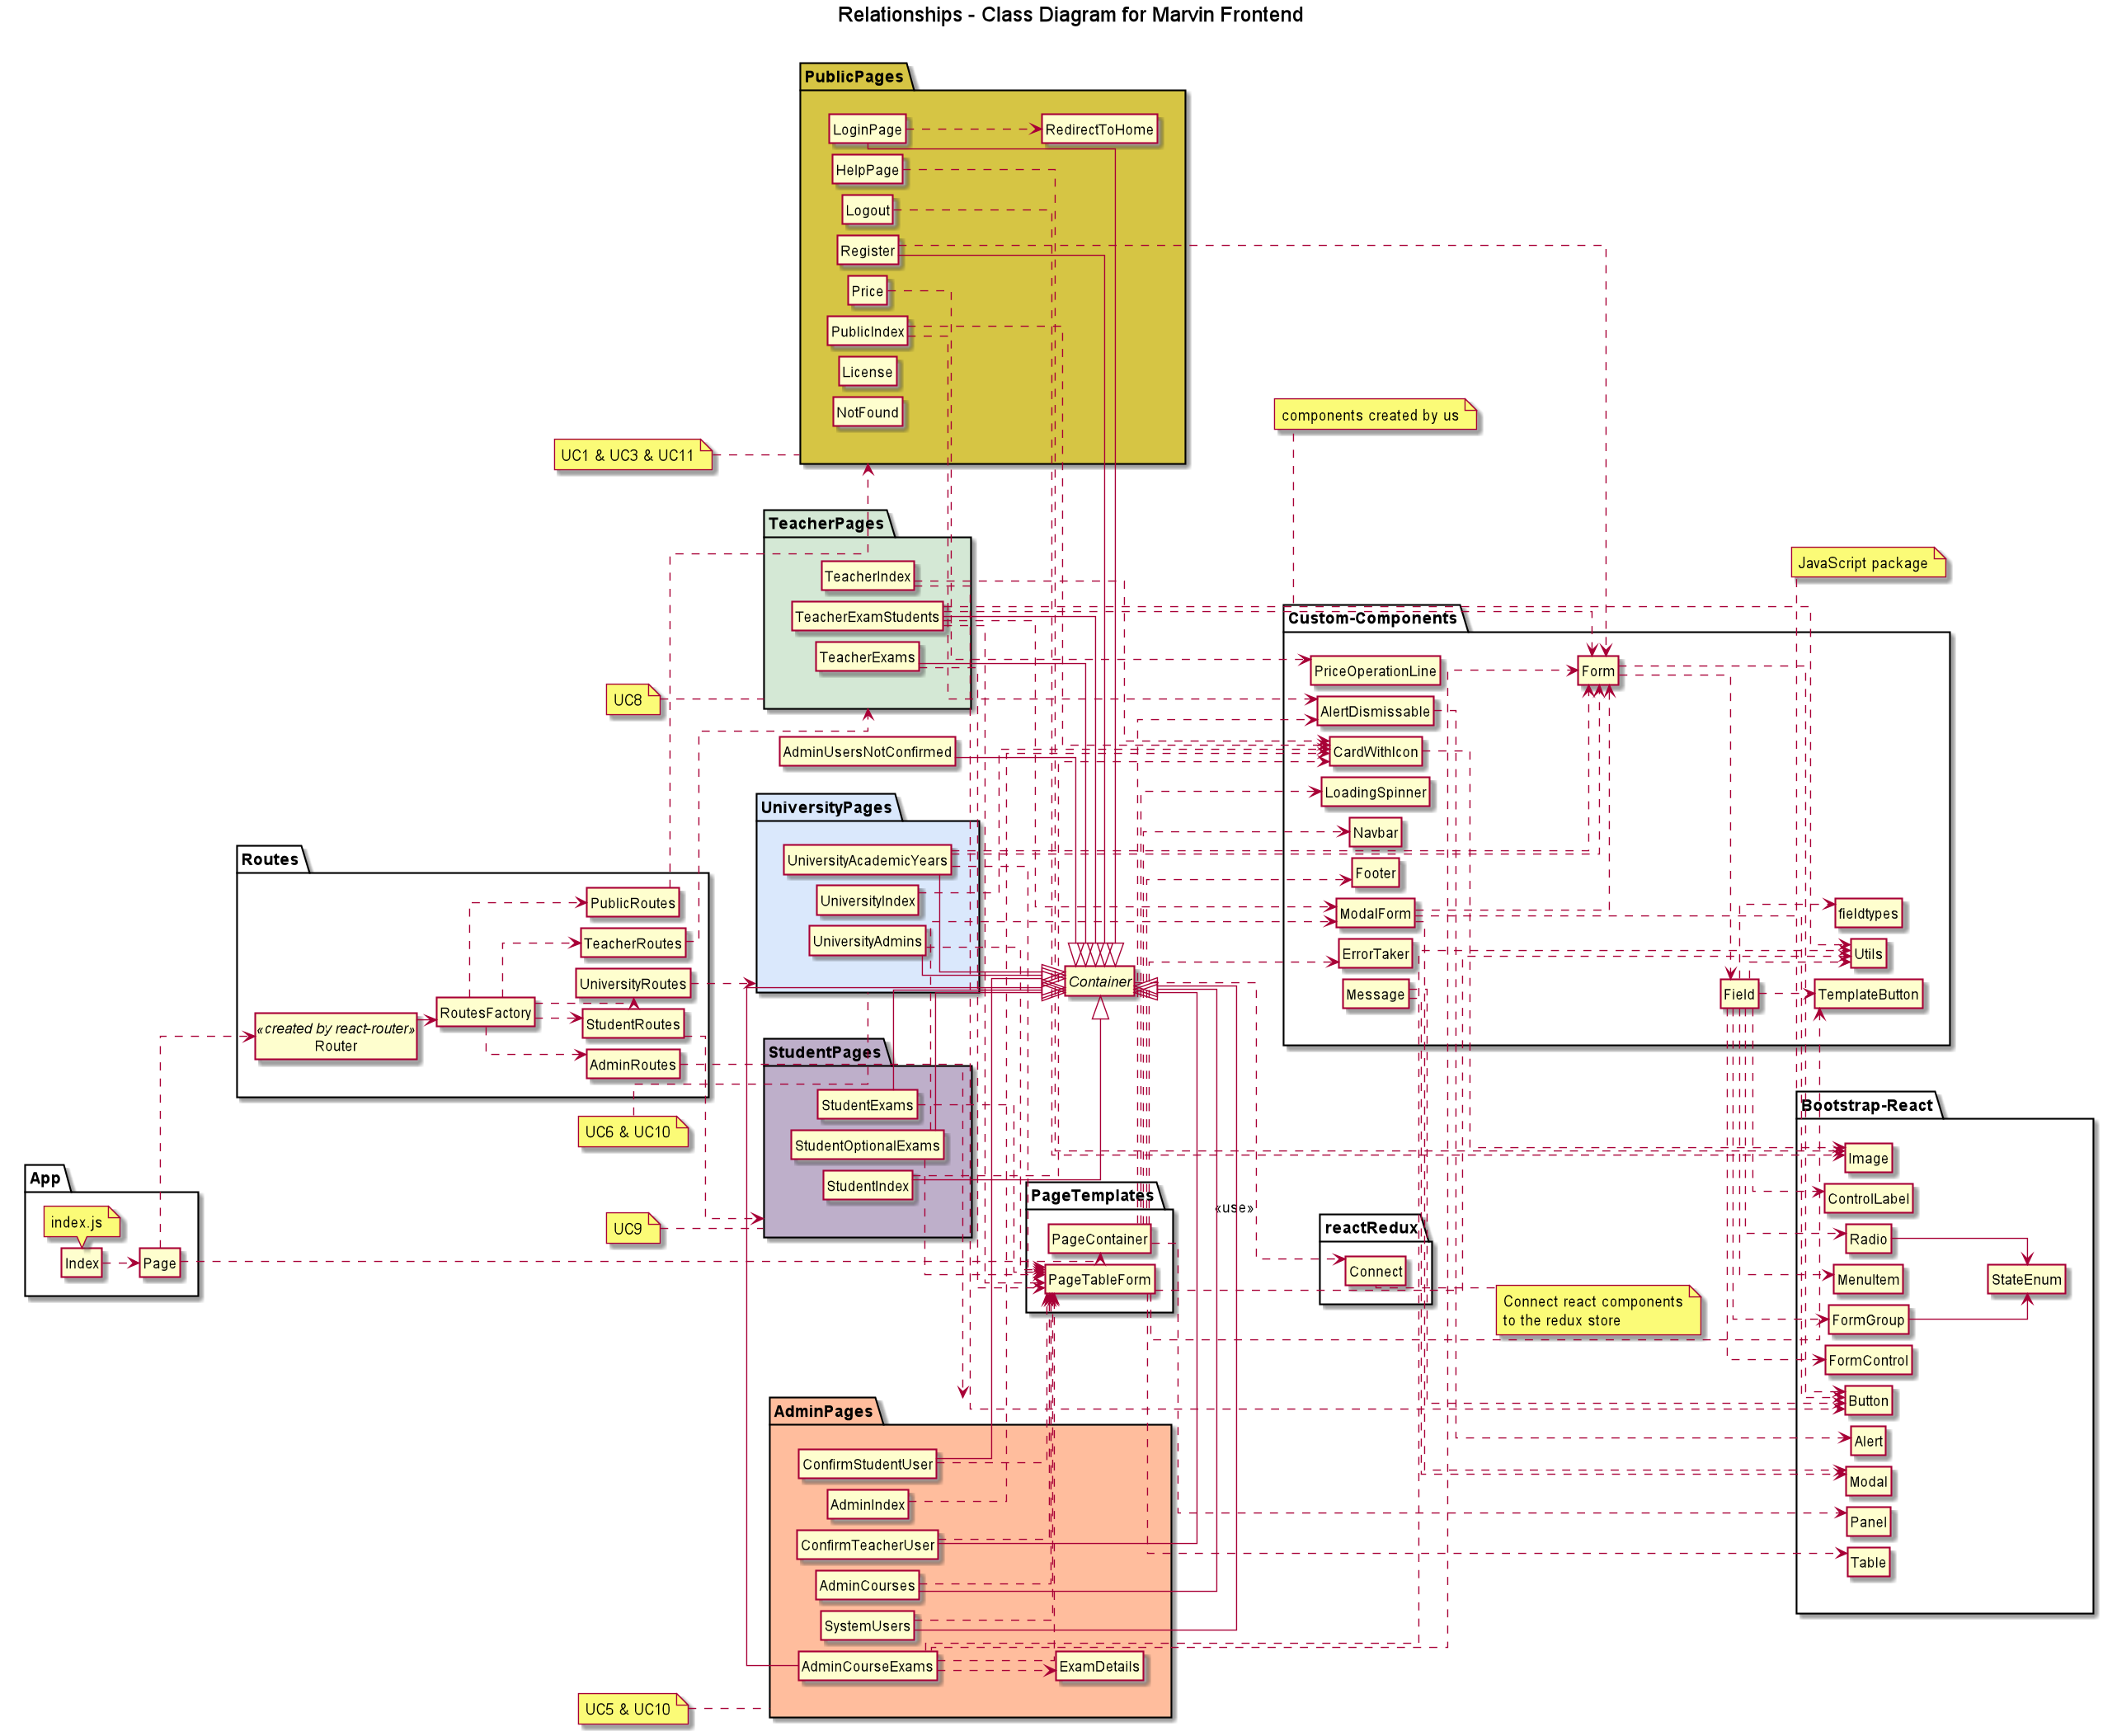
\includegraphics[width=1\linewidth]{"../diagrammi/react/arch."}
		\caption{Entire React Architecture}
		\label{fig:Entire React Architecture}
	\end{figure}
\end{document}